\newpage
\section{Detektion von Snooker-Kugeln}\label{kap:detektion}
Aufgrund eines Bildes des Billardtisches soll der Spielstand mit der Position aller Kugeln bestimmt werden.
Der in dieser Arbeit verwendete Detektionsalgorithmus stammte von der vorherigen Projektarbeit\cite{project2:snooker_detection}
und funktioniert für Snooker-Kugeln.
In der Vorarbeit wurde die Detektion dafür vorgesehen, per Knopfdruck durchgeführt werden konnte.
Mit dieser Arbeit wurde darauf aufbauend eine Live-Detektion implementiert, welche kontinuierlich Bilder vom Tisch macht,
den Spielstand detektiert und dem Benutzer über den Projektor anzeigt.
Dadurch entsteht ein Feedback-Loop, weil die dargestellten Augmentationen im Bild, das verarbeitet wird, ersichtlich sind.
Ein Eingabebild für die Detektion ist in Abbildung \ref{fig:detection_feedback_loop} dargestellt und zeigt diesen Feedback-Loop.

\begin{figure}[h!]
    \begin{center}
        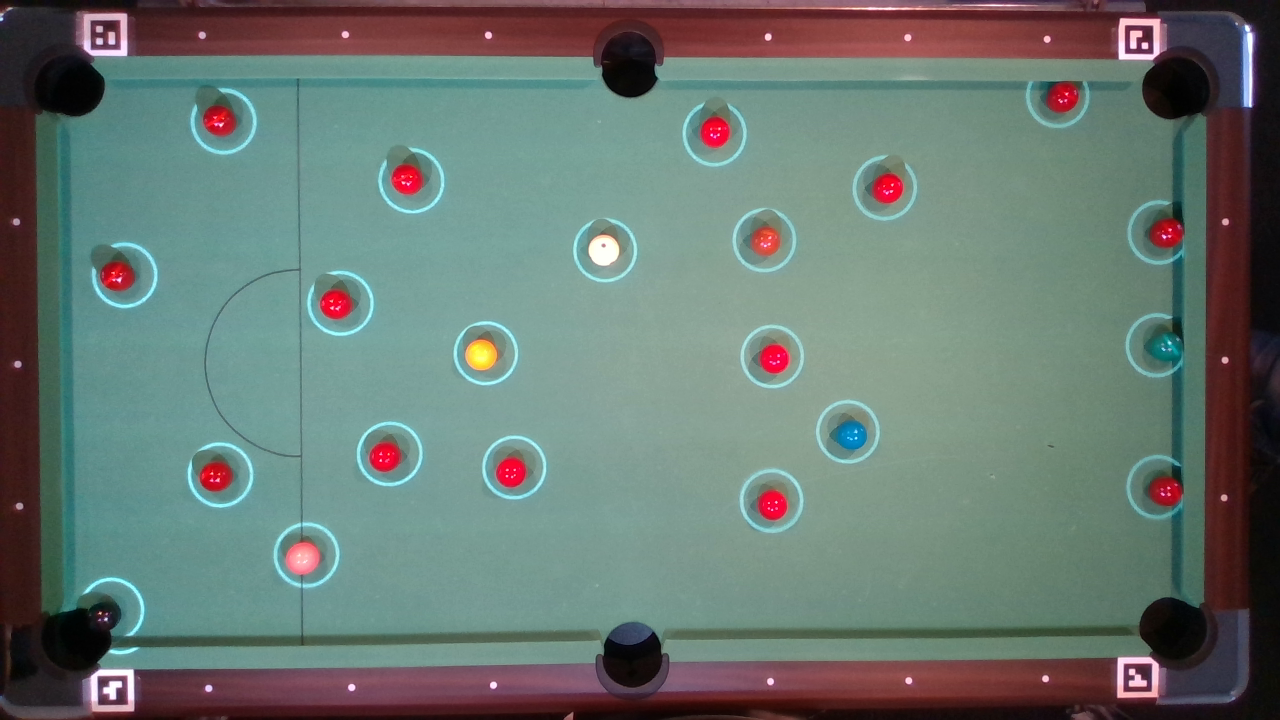
\includegraphics[width=0.8\linewidth]{../common/03_billiard_ai/resources/detection_feedback_loop.png}
    \end{center}
    \caption{Feedback-Loop in der Detektion}
    \label{fig:detection_feedback_loop}
\end{figure}

Die dargestellten Augmentationen könenn zu fälschlicherweise detektierten Kugeln führen.
Um diesem Problem entgegenzuwirken wurden die Parameter der Detektion angepasst, damit die Augmentationen grösstenteils
entfernt werden können. Da allerdings nicht alle restlos entfernt werden können, besteht ein Restrisiko für
fälschlicherweise detektierte Kugeln.

Des Weiteren wurde die Performance der Detektion erhöht, um die Live-Detektion aufzuwerten.
In der bisherigen Detektion wurden drei separate Circle Hough transform\cite{wiki:circle_hough} angewendet, eine für
jede der drei Gruppen von Kugeln, in die das Bild mittels Segmentation aufgeteilt wurde\cite{project2:snooker_detection}.
Zwei dieser drei konnten ohne einen bemerkbaren Verlust in der Qualität der Detektion zusammengefasst werden.
